\documentclass[12pt,letterpaper]{article}
\usepackage{fullpage}
\usepackage[top=2cm, bottom=4.5cm, left=2.5cm, right=2.5cm]{geometry}
\usepackage{amsmath,amsthm,amsfonts,amssymb,amscd}
\usepackage{lastpage}
\usepackage{enumerate}
\usepackage{fancyhdr}
\usepackage{mathrsfs}
\usepackage{xcolor}
\usepackage{graphicx}
\usepackage{listings}
\usepackage{hyperref}
\usepackage{soul}
\usepackage{pgfplots}

\hypersetup{%
  colorlinks=true,
  linkcolor=blue,
  linkbordercolor={0 0 1}
}
 
\renewcommand\lstlistingname{Algorithm}
\renewcommand\lstlistlistingname{Algorithms}
\def\lstlistingautorefname{Alg.}

\lstdefinestyle{Python}{
    language        = Python,
    frame           = lines, 
    basicstyle      = \footnotesize,
    keywordstyle    = \color{blue},
    stringstyle     = \color{green},
    commentstyle    = \color{red}\ttfamily
}

\setlength{\parindent}{0.0in}
\setlength{\parskip}{0.05in}

% Edit these as appropriate
\newcommand\course{CSCI 3104}      %<--class
\newcommand\hwnumber{1}                  % <-- homework number
\newcommand\NetIDa{Rhett Hanscom}           % <-- NetID of person #1
\newcommand\NetIDb{rhha1623@colorado.edu}           % <-- NetID of person #2 (Comment this line out for problem sets)

\pagestyle{fancyplain}
\headheight 35pt
\lhead{\NetIDa}
\lhead{\NetIDa\\\NetIDb}                 % <-- Comment this line out for problem sets (make sure you are person #1)
\chead{\textbf{\Large Homework \hwnumber}}
\rhead{\course \\ \today}
\lfoot{}
\cfoot{}
\rfoot{\small\thepage}
\headsep 1.5em

\begin{document}

\section*{Problem 1}

The Netflix recommendation system uses three main structures to curate a unique profile for each user. These are:
\begin{enumerate}
  \item
   The User - and the direct data they provide (i.e., what is watched, when it is watched, how they have rated media, etc.)
  \item
    Taggers - people paid to watch and tag all the media on Netflix with the media's unique identifiers
  \item
    Machine Learning Algorithm - ties everything together
\end{enumerate}
 
 Netflix uses the user data to create communities of users who watch similar tags frequently. There are more than 2,000 unique communities currently and a single user can reside in multiple communities concurrently. 
 
 The machine learning algorithm at the heart of this process creates something similar to a weighted graph which places users with similar tag histories in clusters. forming the mentioned `communities'. Media eliciting a positive response is shared with nearby located users. This is how the Netflix recommendation system works in a nutshell.
 
%    Here is an example typesetting mathematics in \LaTeX
%\begin{equation*}
%    X(m,n) = \left\{\begin{array}{lr}
%        x(n), & \text{for } 0\leq n\leq 1\\
%        \frac{x(n-1)}{2}, & \text{for } 0\leq n\leq 1\\
%        \log_2 \left\lceil n \right\rceil \qquad & \text{for } 0\leq n\leq 1
%        \end{array}\right\} = xy
%\end{equation*}
%
%    \item Problem 1 part 3 answer here.
%
%    Here is an example of how you can typeset algorithms.
%    There are many packages to do this in \LaTeX.
%     
%    \lstset{caption={Caption for code}}
%    \lstset{label={lst:alg1}}
%     \begin{lstlisting}[style = Python]
%    from package import Class # Mesh required for..
%    
%    cinstance = Class.from_obj('class.obj')
%    cinstance.go()
%    \end{lstlisting}
%     
%  \item Problem 1 part 4 answer here.
%
%    Here is an example of how you can insert a figure.
%    \begin{figure}[!h]
%    \centering
%    \includegraphics[width=0.3\linewidth]{heidi.jpg}
%    \caption{Heidi attacked by a string.}
%    \end{figure}
%\end{enumerate}
%

\section*{Problem 2}



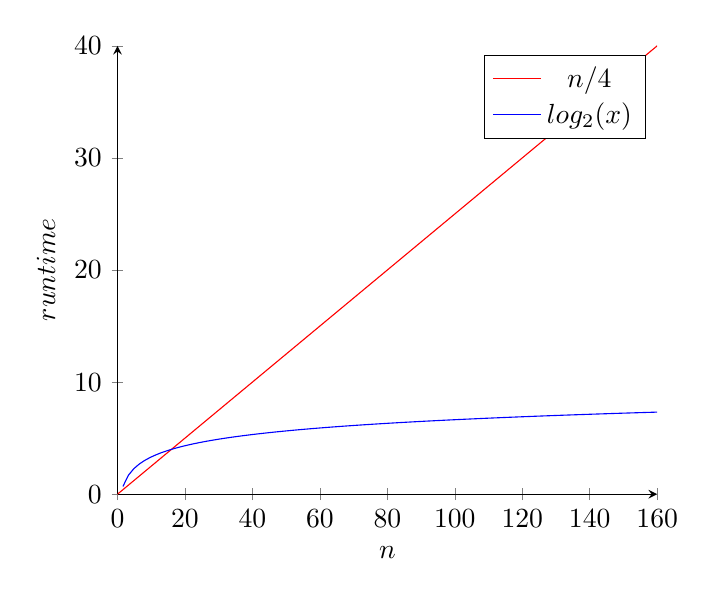
\begin{tikzpicture}
\begin{axis}[
    axis lines = left,
    xlabel = $n$,
    ylabel = {$runtime$},
]
%Below the red parabola is defined
\addplot [
    domain=0:160, 
    samples=100, 
    color=red,
]
{x/4};
\addlegendentry{$n/4$}
%Here the blue parabloa is defined
\addplot [
    domain=0:160, 
    samples=100, 
    color=blue,
    ]
    {log2(x)};
\addlegendentry{$log_{2}(x)$}
 
\end{axis}
\end{tikzpicture}


As the above illustration demonstrates, \textit{n/4} is the better algorithm for n \textless{} 16, while \textit{$log_{2}(x)$}{}
is better suited for n \geq{} 16.\end{geg}This is show by the \textit{n/4} line being lower than the \textit{$log_{2}(x)$}{} line 
on this interval, indicating a shorter runtime. At n = 16, the two equations are equivalent with \textit{$16/4$} = \textit{$log_{2}(16)$}{} = 4, 
so from this point on the \textit{$log_{2}(n)$}{} equation would be preferred.


\section*{Problem 3}


\begin{center}
\begin{tabular}{ |c|c|c|c|c|| } 
\hline
Number of Drinks (d) & Number of Patrons (p) & Arnold's Equation & Barry's Equation\\
\hline
5 & 4 & 2.5 & 3.2189 \\ 
10 & 10 & 5 & 4.6052 \\ 
15 & 4 & 7.5 & 5.4161 \\ 
20 & 8 & 10 & 5.9915 \\
\hline
\end{tabular}
\end{center}

\begin{center}
\begin{tabular}{ |c|c|} 
\hline
Arnold's \vert{} Error \vert{} & Barry's \vert{} Error \vert{} \\
\hline
1.5 & .8 \\ 
5 & 5.4 \\
3.5 & 1.4 \\
2 & 2.1 \\
\hline
\end{tabular}
\end{center}


\begin{center}
\begin{tabular}{ |c|c|} 
\hline
Arnold's Total \vert{} Error \vert{}  & Barry's Total \vert{} Error \vert{} \\
\hline
12 & 9.7 \\
\hline
\end{tabular}
\end{center}

I would argue that Barry's equation of \textit{2ln(d)} is the more accurate for this small data set. I determined this by summing the absolute value of the error between each Arnold and Barry's equation inputs and the actual number of patrons. The total sum of \vert{} error \vert{} \end w was less for Barry and his algorithm, therein he had the more accurate algorithm (still not great though!).


\section*{Problem 4}

\begin{enumerate}
\item
\begin{verbatim}
int Function (int n){
    int Sequence[n];
  if (n == 0){return 1;} else {Sequence[0] = 1;}
  if (n == 1){return -1;} else {Sequence[1] = -1;}
  if (n == 2){return 2;} else {Sequence[2] = 2;}
  for(int i = 3;  i < n ; i++){
    Sequence[i] = ((Sequence[i-1]*Sequence[i-2]) + Sequence[i-3]);
  }
  return Sequence[n-1];}
\end{verbatim}

\item
The 10th number in the sequence (with an index of 9) is -110,655. This as demonstrated by the following table: 

\begin{center}
\begin{tabular}{ |c|c|} 
\hline
n & G_{n} \\
\hline
0 & 1\\
1&-1\\
2&2\\
3&-1\\
4&-3\\
5&5\\
6&-16\\
7&-83\\
8&1333\\
9&-110,655\\
10&-147,503,281\\

\hline
\end{tabular}
\end{center}

\end{document}